% Para documento texto corto
%\documentclass[paper=letter,oneside,fontsize=12pt]{article}
\documentclass[paper=letter,oneside,fontsize=11pt, parskip=full]{scrartcl}
%\documentclass[paper=letter,oneside,fontsize=12pt]{scrartcl}

% Establece dimensiones de los margenes
% \usepackage[inner=1.5cm,outer=3cm,top=2cm,bottom=4cm,
% bindingoffset=5mm]{geometry}
\usepackage[left=3cm,right=3cm,top=3cm,bottom=3cm,
bindingoffset=0cm, footskip=0.5cm, headheight=2cm]{geometry}

% Elimina sangrias y aumenta espacio entre parrafos
\usepackage{parskip}

% Permite cambiar margenes derecho e izquierdo
% de secciones de texto con el entorno
% adjustwidth
\usepackage{changepage}

% Permite establecer el espaciado entre lineas
\usepackage{setspace}

% Permite ingresar caracteres acentuados y especiales 
% sin necesidad de emplear comando
% utf8 codificacion de entrada Unicode (mas simbolos que ASCII)
\usepackage[utf8]{inputenc}

% Formato direccione URL
% \usepackage{hyperref}

% T1 encoding for European, English, American text
\usepackage[T1]{fontenc}
% Fuente escalable
% \usepackage{lmodern}

% Reemplazo para fuente Arial
\usepackage{helvet}
% Usa la fuente sans-serif por defecto
\renewcommand{\familydefault}{\sfdefault}

% Carga babel, idioma ingles
\usepackage[english,spanish]{babel}

% Mejor jsutificacion, tipografia alta calidad.
\usepackage{microtype}
% Para unir columnas y filas en tablas
\usepackage{array}

% Agrega comandos extra al comando tabular
% \toprule, \midrule, \bottomrule
\usepackage{booktabs}
% Tablas con ancho establecido por usuario
\usepackage{tabularx}
% Para posicionamiento preciso de tablas dentro del texto
\usepackage{float}

% Encabezados personalizados
\usepackage{fancyhdr}
\usepackage{graphicx}

% Permite obtener el numero de la ultima pagina
\usepackage{lastpage}

% Paquetes para figuras
% Paquete caption para titulos figuras
% Paquete subcaption para subfiguras
\usepackage{caption}
\usepackage{subcaption}

% Espaciado inteligente
\usepackage{xspace} 

% Para formato de codigo fuente
\usepackage{xcolor}
\usepackage{listings}
\lstset{basicstyle=\ttfamily,
	showstringspaces=false,
	commentstyle=\color{red},
	keywordstyle=\color{blue}}

% Cabeceras
\pagestyle{fancy}
% Borra cabecera y pie actuales
\fancyhead{}
% Cintillo cabecera
%\chead{
%	
\includegraphics[width=150mm]{Imagenes/Cabecera.png}
%}
\fancyhead[L]{\includegraphics[width=0.3\textwidth]{Imagenes/cabecera.pdf}}
\fancyfoot[C]{ 
	\begin{tabularx}{\textwidth}{|m{3.0cm}|X|m{2.5cm}|m{1.0cm}|}
		\hline			
			\centering
			\includegraphics[height=0.8cm]{Imagenes/pie-izq.pdf} &			
			\centering
			Confidencial &
			\centering
			\includegraphics[height=0.8cm]{Imagenes/pie-der.pdf}  &			
			\thepage~/~\pageref{LastPage} \\
		\hline 
	\end{tabularx}	 
}

% Comando para formatear y justificar parrafos de código y 
% comandos de shell
% \newcommand{\code}[1]{
%	\begin{adjustwidth}{1.5cm}{0.0cm}
%		\ttfamily
%		#1
%	\end{adjustwidth}}	

% Entorno para formato de secciones de codigo
\newenvironment{code}
	{\begin{adjustwidth}{1.5cm}{0.0cm}\ttfamily}
	{\end{adjustwidth}}

% Entorno para formato de secciones de enlaces
\newenvironment{link}
	{\ttfamily}{}

% Numeracion de paginas
% numeros arabigos
\pagenumbering{arabic}

	\begin{document}
			
		%\begin{titlepage}
		
		\begin{center}		
			
			\vspace{10cm}
			% 12 puntos = fuente large
			\begin{large}
				\bfseries
				\uppercase{Dirección de Servicios de Certificación}			
				\vspace{5pt}
				\begin{spacing}{0.9}
					\uppercase{Laboratorio de Ensayos de Compatibilidad~Electromagnética~Radiada}
				\end{spacing}
			\end{large}
			
			%\vspace{10cm}
			\vfill
			
			% 16 puntos = fuente Large de 14 puntos			
			\begin{Large}
				\bfseries				
				\begin{spacing}{0.9}		
					\uppercase{Instalación de librería VXI-11}
				\end{spacing}
			\end{Large}	
				
			\vspace{5pt}
			
			% 12 puntos fuente large
			\begin{large}						
				\uppercase{Sub Título}
			\end{large}	
			
			\vfill
			
			\begin{table}[!h]
				\begin{tabularx}{\linewidth}{|X|X|X|X|}	
					\hline				
					\multicolumn{2}{|l|}{\textbf{CÓDIGO}: FO-IT-002} & \multicolumn{2}{l|}{\textbf{N DOC:}} \\
					\hline
					Originado por:	& 	Elaborado por: & 
					Revisado por: 	& 	Aprobado por: \\
					\hline
					Br. Arias B., Jose A. & Br. Arias B., Jose A. & - & - \\
					\hline
					\textbf{Fecha: 07/07/2017 } & 
					\textbf{Fecha: 07/07/2016} & 
					\textbf{Fecha: } &
					\textbf{Fecha: } \\				
					\hline
				\end{tabularx}	
			\end{table}	
			
			%\vspace{10mm}			
			\vfill
		
		\end{center}
	
	%\end{titlepage}
	
	\clearpage
	
	\tableofcontents
	
	\section{Objetivos}
		\begin{itemize}
			\item Describir el acceso a instrumentos de medición por medio del puente LAN/GPIB E5810
		
		\end{itemize}
		
	\section{Alcance}
	
		En este documento se explica como establecer un puente de conexión entre instrumentos de medición GPIB y una red LAN. Para ello se estblecerá la configuración del puente LAN/GPIB Agilent E5810A. Se detallará principalmente la instalación de la libreria VXI-11 para linux, soporte de software que permite el acceso programático a este dispositivo.	
		
	\section{Documentos de referencia}
	
		\subsection{Enlances de interés}

	
			\begin{link}

			\end{link}	
	

	
	\section{Términos y definiciones}
	
		\begin{tabular}{rl}
			Termino 	& 	Definición \\	
			VXI			& 	VMEbus eXtensions for Instrumentation \\
		\end{tabular}
	
	\section{Personal autorizado}	
		\label{Sec:PersonalAutorizado}		
		Personal técnico del Cendit con interés en el acceso a instrumentos de medición GPIB por medio de un puente de redes LAN a GPIB.
		
	\section{Personal requerido}	
		
		Ver sección \ref{Sec:PersonalAutorizado}.
		
	\section{Materiales}
	
		\label{Sec:SeccionMateriales}
		\begin{itemize}
			\item Computador con acceso a internet.
			\item Puente LAN/GPIB Agilent E5810A.
			\item Cable ethernet cruzado.
		\end{itemize}	
			
	\section{Herramientas y equipos}
		
		Ver sección \ref{Sec:SeccionMateriales}.

	
	\section{Equipos de protección personal}
	
		No se requieren equipos protección personal.
		
	\section{Precauciones de seguridad}
	
		Para ejecutar esta actividad no se preveen precauciones de seguridad
		
	\section{Descripción de la actividad}
	
		\subsection{Generalidades}
				
		\begin{figure}[!h]
			\begin{center}
				%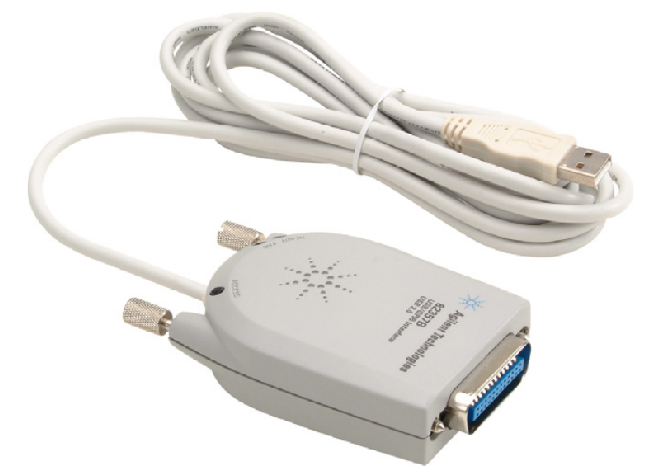
\includegraphics[width=10cm]{Imagenes/AdaptadorGpibUsb.pdf}
				\caption{Adaptador USB GPIB 82357B de Agilent Technologies}
				\label{Fig:AdaptadorGpibUsb}
			\end{center}
		\end{figure}	
		
	
		

	
		\subsection{Instalación de linux-gpib y módulos de núcleo}		
		
		\subsection{Instalación de módulos de núcleo}	
		
		\subsection{Instalación de archivos binarios de firmware para el 82357B}	

			
	\section{Anexos}	
		
		\subsection{Script de Bash para carga automática de firmware}
	
			\begin{lstlisting}[language=c,caption={Listado programa}]
	
#include <stdlib.h>
#include <stdio.h>

int main()
{
	printf("Hola Gafo");
	
	return 0;
}

		\end{lstlisting}
\end{document}